All results are from offline simulation. Each value is computed by the scripts in the supplementary archive from stored raw logs; no value was entered by hand.

\subsection{Tier-1 Performance of the A-DO-SMC}\label{sec:res_tier1}
\begin{table*}[t]
\centering\footnotesize\setlength{\tabcolsep}{5pt}
\caption{Tier-1 comparison on held-out drive cycles of the Tesla Model 3 plant (fixed supervisor, mean over noise seeds 101--103). The last column is the median time of one controller update on the simulation host.}
\label{tab:tier1}
\begin{tabular}{@{}lccccccc@{}}
\toprule
 & \multicolumn{2}{c}{US06} & \multicolumn{2}{c}{US06$\times1.1$} & \multicolumn{2}{c}{WLTC x-high$\times1.2$} & Update\\
Outer loop & max$|e|$ (V) & RMS $e$ (V) & max$|e|$ (V) & RMS $e$ (V) & max$|e|$ (V) & RMS $e$ (V) & (\si{\micro s})\\
\midrule
PI (same small-signal poles) & 8.47 & 0.628 & 9.30 & 0.690 & 0.63 & 0.090 & \TimePI\\
DO-SMC, low gain ($k_s=120$\,V/s) & 6.95 & 0.367 & 7.75 & 0.421 & 0.18 & 0.033 & \TimeDOSMC\\
DO-SMC, high gain ($k_s=\KsHi$\,V/s) & 1.48 & 0.043 & 1.63 & 0.045 & 0.18 & 0.033 & \TimeDOSMC\\
Robust MPC (offset-free, $N=20$) & 1.48 & 0.044 & 1.63 & 0.045 & 0.18 & 0.034 & \TimeMPC\\
A-DO-SMC (proposed tier 1) & 1.48 & 0.043 & 1.63 & 0.045 & 0.18 & 0.033 & \TimeADOSMC\\
\bottomrule
\end{tabular}
\end{table*}


Table~\ref{tab:tier1} compares five outer loops on the Tesla Model 3 plant with the fixed supervisor, on the three test items with the largest bus deviations.

\paragraph{Fixed low gain}
With $k_s=\SI{120}{V/s}$, the observer error on US06 reaches $|\Dt|_{\max}=\DtLoUSnn$\,V/s in the noise-free run, about \DtLoRatio\ times the switching gain. The reaching condition $k_s>|\Dt|$ holds in steady state (\CondLoFrac\,\% of the samples) but is violated during the strong acceleration and braking transients. Outside the boundary layer the switching term then contributes at most $C_{dc}k_s\approx\SI{0.56}{A}$, and the loop reduces to observer compensation plus the $c_ve$ term. The maximum bus deviation on US06 is \TOneLoUSMax\,V, closer to a PI controller with the same small-signal poles (\TOnePIUSMax\,V) than to the robust MPC (\TOneMPCUSMax\,V).

\paragraph{Adaptive gain}
A-DO-SMC lowers the maximum deviation on US06 to \TOneAUSMax\,V and the RMS deviation from \TOneLoUSRms\ to \TOneAUSRms\,V, the same as the robust MPC, whose QP constraints were never active in these runs, so the MPC acts as an observer-compensated LQR. On US06$\times1.1$ the values are \TOneAUSbMax\,V against \TOneLoUSbMax\,V. On the WLTC cycles all observer-based loops reach about \SI{0.2}{V}, and only PI is worse.

\paragraph{Fixed high gain}
A fixed gain sized for the worst case of the training cycles ($k_s=\KsHi$\,V/s, $\phi_s=\PhiHi$\,V) satisfies the reaching condition on US06 (\CondHiFrac\,\% of the samples, minimum ratio $k_s/|\Dt|=\CondHiMin$) and gives the same regulation as A-DO-SMC on every test item (Table~\ref{tab:tier1}). On the nominal plant, the benefit of A-DO-SMC is therefore not better regulation than a well-sized constant gain. It lies in three properties: the gain does not have to be sized in advance from a worst-case error bound; the condition is enforced for whatever observer gain $\lambda$ a supervisor applies, whereas a fixed gain sized at the nominal $\lambda$ loses its margin when $\lambda$ is lowered, because the bound \eqref{eq:ndobound} on $|\Dt|$ grows as $\rho_D/\lambda$; and the large gain and wide boundary layer are applied only while the observer error is large. At the nominal observer gain the high-gain margin on US06 is small (\CondHiMin); its consequence is tested next.

\paragraph{Robustness to the observer gain}
\begin{table*}[t]
\centering\footnotesize\setlength{\tabcolsep}{4pt}
\caption{Robustness of tier 1 to the observer gain on US06 (Tesla Model 3 plant). Hi: fixed high-gain DO-SMC ($k_s=\KsHi$\,V/s, sized at the nominal $\lambda=\SI{250}{s^{-1}}$); A: A-DO-SMC. Agent rows replay open-loop the schedule $(\tau_b,v_{sc,ref},\lambda)(t)$ chosen by each filter-v2 agent in its evaluation run, so both controllers see the same $\lambda(t)$. max$|e|$: mean over noise seeds 101--103; $r_{\min}=\min_t k_s/|\Dt|$ ($t>0.2$\,s, seed 101, \SI{1}{ms} logging). $^\ddagger$Power deficit (input saturated \LamSatPct\,\% of the time, capability condition (H3) violated).}
\label{tab:lambda}
\begin{tabular}{@{}llcccccccc@{}}
\toprule
 & & \multicolumn{4}{c}{US06} & \multicolumn{4}{c}{US06$\times1.1$}\\\cmidrule(lr){3-6}\cmidrule(lr){7-10}
$\lambda$ schedule & $\lambda$ range (s$^{-1}$) & \multicolumn{2}{c}{max$|e|$ (V)} & \multicolumn{2}{c}{$r_{\min}$} & \multicolumn{2}{c}{max$|e|$ (V)} & \multicolumn{2}{c}{$r_{\min}$}\\
 & & Hi & A & Hi & A & Hi & A & Hi & A\\
\midrule
constant, $\lambda=\lambda_{\min}$ & 100 & 11.40 & 2.71 & 0.554 & 1.316 & 12.04 & 2.98 & 0.508 & 1.320\\
constant, nominal & 250 & 1.48 & 1.48 & 1.101 & 1.252 & 1.63 & 1.63 & 1.026 & 1.250\\
constant, $\lambda=\lambda_{\max}$ & 800 & 0.59 & 0.59 & 2.144 & 1.032 & 0.64 & 0.64 & 2.070 & 1.025\\
\midrule
TD3 agent, seed 11 & 114--746 & 1.58 & 1.58 & 1.167 & 1.090 & 1.96 & 1.96 & 0.997 & 1.093\\
TD3 agent, seed 22 & 121--800 & 0.90 & 0.90 & 1.926 & 1.147 & 0.97 & 0.97 & 1.818 & 1.004\\
TD3 agent, seed 33 & 133--800 & 1.03 & 1.03 & 1.733 & 1.028 & 167.98$^\ddagger$ & 167.85$^\ddagger$ & 0.040 & 0.047\\
\bottomrule
\end{tabular}
\end{table*}

Table~\ref{tab:lambda} tests this property on US06, with the observer gain held at the bounds of the safety filter and at its nominal value, and with the $\lambda$ schedules chosen by the three filter-v2 agents.
\begin{itemize}
\item \emph{Lower bound} ($\lambda=\SI{100}{s^{-1}}$). The observer error grows, and the fixed high gain no longer satisfies the reaching condition ($r_{\min}=\LamHiUSRatio$). The condition fails in only \LamHiUSFail\,\% of the samples, yet the maximum bus deviation rises to \LamHiUSMax\,V (\LamHiUSbMax\,V on US06$\times1.1$). A-DO-SMC raises its gain with the error ($r_{\min}=\LamAUSRatio$) and limits the deviation to \LamAUSMax\,V, \LamFactorHi\ times less.
\item \emph{Nominal value and upper bound.} Both controllers give identical regulation. Whenever the reaching condition holds, both operate inside the boundary layer with the same slope $k'$, so their closed loops coincide.
\item \emph{Agent schedules.} Replaying the agents' schedules open-loop gives identical regulation for both controllers (largest difference \LamAgentMaxDiff\,V outside the deficit run). The agents lowered $\lambda$ to \LamAgentMin\,s$^{-1}$ only briefly and kept it at \LamAgentMeanLo--\LamAgentMeanHi\,s$^{-1}$ on average, above the nominal value. The fixed high gain therefore violated the condition only marginally ($r_{\min}=\LamHiAgentRatioMin$, seed 11 on US06$\times1.1$) and without visible effect. The power deficit of the seed-33 schedule on US06$\times1.1$ violates the capability condition (H3) and affects both controllers equally.
\end{itemize}
The robustness of A-DO-SMC to the observer gain is thus decisive when $\lambda$ is low during strong transients, as at the lower filter bound; the evaluated agents did not operate there, so in the agent runs it was not exercised. With noise, A-DO-SMC kept $k_s\ge|\Dt|$ in all runs without a deficit ($r_{\min}\ge\LamARatioMin$). Several of these ratios are below the value $12/11$ used in Section~\ref{sec:tier1}, so the numerical check of Assumption~\ref{as:est} is not met in every noisy run.

\paragraph{Gain-adaptation mechanism}
Fig.~\ref{fig:tier1} shows the largest transient of US06. In the noise-free run, the envelope raises $k_s(t)$ to $\KsMaxAdapt$\,V/s, above the true observer error ($|\Dt|_{\max}=\DtildeMaxAdapt$\,V/s). The condition $k_s\ge|\Dt|$ holds during \AssumptionHoldPct\ of the run, with a minimum ratio $k_s/|\Dt|$ of \MinKsRatio; since this ratio exceeds $12/11$, Assumption~\ref{as:est} is satisfied in this run (Section~\ref{sec:tier1}). With measurement noise the condition also holds in all logged samples (\SI{1}{ms} resolution, minimum ratio \AsmNoisyMinRatio). In steady state the gain decays toward $k_{\min}$, and the boundary layer $\phi_s=k_s/k'$ shrinks with it. The control law is therefore never high-gain inside the layer: its slope stays at $k'=\SI{240}{s^{-1}}$ throughout.

\paragraph{Computational cost}
One A-DO-SMC update costs \TimeADOSMC\,\si{\micro s}, essentially the same as a fixed-gain DO-SMC (\TimeDOSMC\,\si{\micro s}). The robust MPC costs \TimeMPC\,\si{\micro s} when its constraints are inactive and \TimeMPCActive\,\si{\micro s} when they are active.

\begin{figure*}[t]
\centering
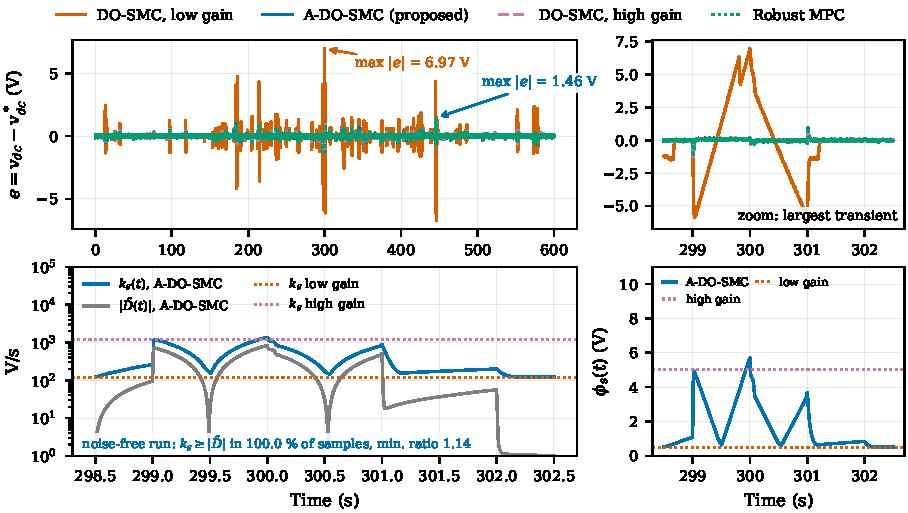
\includegraphics[width=\textwidth]{../results/figures/F2_tier1_m3_us06.pdf}
\caption{US06 on the Tesla Model 3 plant, fixed supervisor, noise seed 101. Top: bus-voltage error for the fixed-gain DO-SMC with low and high gain, the robust MPC and A-DO-SMC over the whole cycle (left) and around the largest transient (right, \ZoomA--\ZoomB\,s). The high-gain DO-SMC and robust MPC curves lie on that of A-DO-SMC. Bottom (noise-free run of A-DO-SMC, same window): adaptive switching gain $k_s(t)$ and true observer error $|\Dt(t)|$, computed from the plant (left, log scale), and boundary-layer width $\phi_s(t)=k_s(t)/k'$ (right); dotted lines: the constant values of the two fixed-gain tunings.}
\label{fig:tier1}
\end{figure*}

\subsection{Tier 2: training and validation}\label{sec:res_train}
\begin{figure}[t]
\centering
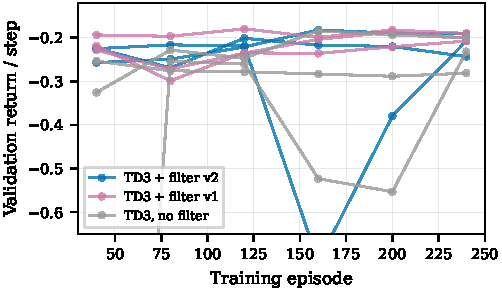
\includegraphics[width=\columnwidth]{../results/figures/F3_validation_curves.pdf}
\caption{Validation return per decision during training (three seeds per variant; evaluated every 40 episodes on WLTC low, WLTC medium, and WLTC medium$\times1.6$). For reference, the fixed and SOC-rule supervisors score \ValFixed\ and \ValRule. Two evaluations fall below the plotted range (no-filter seed 33 at episode 40; filter-v2 seed 33 at episode 160).}
\label{fig:val}
\end{figure}

Fig.~\ref{fig:val} shows the validation return during training. With checkpoint selection on validation only, the selected agents score:
\begin{itemize}
\item filter v2: \ValVtwoSA, \ValVtwoSB, \ValVtwoSC\ (seeds 11, 22, 33);
\item filter v1: \ValVoneSA, \ValVoneSB, \ValVoneSC;
\item no filter: \ValNofSA, \ValNofSB, \ValNofSC.
\end{itemize}
For comparison, the SOC rule scores \ValRule\ and the fixed supervisor \ValFixed. The curves are not monotonic, and one seed of each of the no-filter and v2 variants has a transient collapse. Validation alone would therefore suggest that every filtered agent beats the fixed and rule-based supervisors. The same validation protocol, however, ranks the non-learning MPC-EMS above every agent: \ValMPCPTwo\ with the causal persistence forecast and \ValMPCVTwo\ with preview (Section~\ref{sec:setup}). The test results below show that neither ranking transfers to all unseen cycles.

\subsection{Tier 2: held-out test cycles}\label{sec:res_test}
\begin{table*}[t]
\centering\footnotesize\setlength{\tabcolsep}{4pt}
\caption{Held-out test cycles. Tier~1 is A-DO-SMC in every row. Learned supervisors: mean $\pm$ standard deviation over three training seeds, each value averaged over three noise seeds. Non-learning supervisors: mean over the same three noise seeds. $^\dagger$Non-causal: uses the true future load. A failed run (bus out of range) is truncated at the failure and included in the means. All indices are computed from true plant signals.}
\label{tab:test}
\resizebox{\textwidth}{!}{%
\begin{tabular}{@{}llrrrrrc@{}}
\toprule
Cycle & Supervisor (tier 1 = A-DO-SMC) & max$|e|$ (V) & RMS $i_b$ (A) & RMS $\dot\imath_b$ (A/s) & Sat. (\%) & min $v_{sc}$ (V) & Failed runs\\
\midrule
US06 & Fixed $\theta$ & \R{us06a:afix:maxdev} & \R{us06a:afix:ibrms} & \R{us06a:afix:slew} & \R{us06a:afix:sat} & \R{us06a:afix:vmin} & \R{us06a:afix:fails}/\R{us06a:afix:runs}\\
 & SOC rule~\cite{nguyen2021adaptive} & \R{us06a:arule:maxdev} & \R{us06a:arule:ibrms} & \R{us06a:arule:slew} & \R{us06a:arule:sat} & \R{us06a:arule:vmin} & \R{us06a:arule:fails}/\R{us06a:arule:runs}\\
 & MPC-EMS, persistence & \R{us06a:mpcp:maxdev} & \R{us06a:mpcp:ibrms} & \R{us06a:mpcp:slew} & \R{us06a:mpcp:sat} & \R{us06a:mpcp:vmin} & \R{us06a:mpcp:fails}/\R{us06a:mpcp:runs}\\
 & MPC-EMS, preview$^\dagger$ & \R{us06a:mpcv:maxdev} & \R{us06a:mpcv:ibrms} & \R{us06a:mpcv:slew} & \R{us06a:mpcv:sat} & \R{us06a:mpcv:vmin} & \R{us06a:mpcv:fails}/\R{us06a:mpcv:runs}\\
 & TD3, no filter & \R{us06a:nof:maxdev:mean}\,{\scriptsize$\pm$\R{us06a:nof:maxdev:std}} & \R{us06a:nof:ibrms:mean}\,{\scriptsize$\pm$\R{us06a:nof:ibrms:std}} & \R{us06a:nof:slew:mean}\,{\scriptsize$\pm$\R{us06a:nof:slew:std}} & \R{us06a:nof:sat:mean}\,{\scriptsize$\pm$\R{us06a:nof:sat:std}} & \R{us06a:nof:vmin:mean}\,{\scriptsize$\pm$\R{us06a:nof:vmin:std}} & \R{us06a:nof:fails}/\R{us06a:nof:runs}\\
 & TD3 + filter v1 & \R{us06a:v1:maxdev:mean}\,{\scriptsize$\pm$\R{us06a:v1:maxdev:std}} & \R{us06a:v1:ibrms:mean}\,{\scriptsize$\pm$\R{us06a:v1:ibrms:std}} & \R{us06a:v1:slew:mean}\,{\scriptsize$\pm$\R{us06a:v1:slew:std}} & \R{us06a:v1:sat:mean}\,{\scriptsize$\pm$\R{us06a:v1:sat:std}} & \R{us06a:v1:vmin:mean}\,{\scriptsize$\pm$\R{us06a:v1:vmin:std}} & \R{us06a:v1:fails}/\R{us06a:v1:runs}\\
 & TD3 + filter v2 (prop.) & \R{us06a:v2:maxdev:mean}\,{\scriptsize$\pm$\R{us06a:v2:maxdev:std}} & \R{us06a:v2:ibrms:mean}\,{\scriptsize$\pm$\R{us06a:v2:ibrms:std}} & \R{us06a:v2:slew:mean}\,{\scriptsize$\pm$\R{us06a:v2:slew:std}} & \R{us06a:v2:sat:mean}\,{\scriptsize$\pm$\R{us06a:v2:sat:std}} & \R{us06a:v2:vmin:mean}\,{\scriptsize$\pm$\R{us06a:v2:vmin:std}} & \R{us06a:v2:fails}/\R{us06a:v2:runs}\\
\midrule
WLTC high & Fixed $\theta$ & \R{wh:afix:maxdev} & \R{wh:afix:ibrms} & \R{wh:afix:slew} & \R{wh:afix:sat} & \R{wh:afix:vmin} & \R{wh:afix:fails}/\R{wh:afix:runs}\\
 & SOC rule~\cite{nguyen2021adaptive} & \R{wh:arule:maxdev} & \R{wh:arule:ibrms} & \R{wh:arule:slew} & \R{wh:arule:sat} & \R{wh:arule:vmin} & \R{wh:arule:fails}/\R{wh:arule:runs}\\
 & MPC-EMS, persistence & \R{wh:mpcp:maxdev} & \R{wh:mpcp:ibrms} & \R{wh:mpcp:slew} & \R{wh:mpcp:sat} & \R{wh:mpcp:vmin} & \R{wh:mpcp:fails}/\R{wh:mpcp:runs}\\
 & MPC-EMS, preview$^\dagger$ & \R{wh:mpcv:maxdev} & \R{wh:mpcv:ibrms} & \R{wh:mpcv:slew} & \R{wh:mpcv:sat} & \R{wh:mpcv:vmin} & \R{wh:mpcv:fails}/\R{wh:mpcv:runs}\\
 & TD3, no filter & \R{wh:nof:maxdev:mean}\,{\scriptsize$\pm$\R{wh:nof:maxdev:std}} & \R{wh:nof:ibrms:mean}\,{\scriptsize$\pm$\R{wh:nof:ibrms:std}} & \R{wh:nof:slew:mean}\,{\scriptsize$\pm$\R{wh:nof:slew:std}} & \R{wh:nof:sat:mean}\,{\scriptsize$\pm$\R{wh:nof:sat:std}} & \R{wh:nof:vmin:mean}\,{\scriptsize$\pm$\R{wh:nof:vmin:std}} & \R{wh:nof:fails}/\R{wh:nof:runs}\\
 & TD3 + filter v1 & \R{wh:v1:maxdev:mean}\,{\scriptsize$\pm$\R{wh:v1:maxdev:std}} & \R{wh:v1:ibrms:mean}\,{\scriptsize$\pm$\R{wh:v1:ibrms:std}} & \R{wh:v1:slew:mean}\,{\scriptsize$\pm$\R{wh:v1:slew:std}} & \R{wh:v1:sat:mean}\,{\scriptsize$\pm$\R{wh:v1:sat:std}} & \R{wh:v1:vmin:mean}\,{\scriptsize$\pm$\R{wh:v1:vmin:std}} & \R{wh:v1:fails}/\R{wh:v1:runs}\\
 & TD3 + filter v2 (prop.) & \R{wh:v2:maxdev:mean}\,{\scriptsize$\pm$\R{wh:v2:maxdev:std}} & \R{wh:v2:ibrms:mean}\,{\scriptsize$\pm$\R{wh:v2:ibrms:std}} & \R{wh:v2:slew:mean}\,{\scriptsize$\pm$\R{wh:v2:slew:std}} & \R{wh:v2:sat:mean}\,{\scriptsize$\pm$\R{wh:v2:sat:std}} & \R{wh:v2:vmin:mean}\,{\scriptsize$\pm$\R{wh:v2:vmin:std}} & \R{wh:v2:fails}/\R{wh:v2:runs}\\
\midrule
WLTC extra-high & Fixed $\theta$ & \R{wxa:afix:maxdev} & \R{wxa:afix:ibrms} & \R{wxa:afix:slew} & \R{wxa:afix:sat} & \R{wxa:afix:vmin} & \R{wxa:afix:fails}/\R{wxa:afix:runs}\\
 & SOC rule~\cite{nguyen2021adaptive} & \R{wxa:arule:maxdev} & \R{wxa:arule:ibrms} & \R{wxa:arule:slew} & \R{wxa:arule:sat} & \R{wxa:arule:vmin} & \R{wxa:arule:fails}/\R{wxa:arule:runs}\\
 & MPC-EMS, persistence & \R{wxa:mpcp:maxdev} & \R{wxa:mpcp:ibrms} & \R{wxa:mpcp:slew} & \R{wxa:mpcp:sat} & \R{wxa:mpcp:vmin} & \R{wxa:mpcp:fails}/\R{wxa:mpcp:runs}\\
 & MPC-EMS, preview$^\dagger$ & \R{wxa:mpcv:maxdev} & \R{wxa:mpcv:ibrms} & \R{wxa:mpcv:slew} & \R{wxa:mpcv:sat} & \R{wxa:mpcv:vmin} & \R{wxa:mpcv:fails}/\R{wxa:mpcv:runs}\\
 & TD3, no filter & \R{wxa:nof:maxdev:mean}\,{\scriptsize$\pm$\R{wxa:nof:maxdev:std}} & \R{wxa:nof:ibrms:mean}\,{\scriptsize$\pm$\R{wxa:nof:ibrms:std}} & \R{wxa:nof:slew:mean}\,{\scriptsize$\pm$\R{wxa:nof:slew:std}} & \R{wxa:nof:sat:mean}\,{\scriptsize$\pm$\R{wxa:nof:sat:std}} & \R{wxa:nof:vmin:mean}\,{\scriptsize$\pm$\R{wxa:nof:vmin:std}} & \R{wxa:nof:fails}/\R{wxa:nof:runs}\\
 & TD3 + filter v1 & \R{wxa:v1:maxdev:mean}\,{\scriptsize$\pm$\R{wxa:v1:maxdev:std}} & \R{wxa:v1:ibrms:mean}\,{\scriptsize$\pm$\R{wxa:v1:ibrms:std}} & \R{wxa:v1:slew:mean}\,{\scriptsize$\pm$\R{wxa:v1:slew:std}} & \R{wxa:v1:sat:mean}\,{\scriptsize$\pm$\R{wxa:v1:sat:std}} & \R{wxa:v1:vmin:mean}\,{\scriptsize$\pm$\R{wxa:v1:vmin:std}} & \R{wxa:v1:fails}/\R{wxa:v1:runs}\\
 & TD3 + filter v2 (prop.) & \R{wxa:v2:maxdev:mean}\,{\scriptsize$\pm$\R{wxa:v2:maxdev:std}} & \R{wxa:v2:ibrms:mean}\,{\scriptsize$\pm$\R{wxa:v2:ibrms:std}} & \R{wxa:v2:slew:mean}\,{\scriptsize$\pm$\R{wxa:v2:slew:std}} & \R{wxa:v2:sat:mean}\,{\scriptsize$\pm$\R{wxa:v2:sat:std}} & \R{wxa:v2:vmin:mean}\,{\scriptsize$\pm$\R{wxa:v2:vmin:std}} & \R{wxa:v2:fails}/\R{wxa:v2:runs}\\
\midrule
WLTC extra-high $\times1.2$ & Fixed $\theta$ & \R{wxb:afix:maxdev} & \R{wxb:afix:ibrms} & \R{wxb:afix:slew} & \R{wxb:afix:sat} & \R{wxb:afix:vmin} & \R{wxb:afix:fails}/\R{wxb:afix:runs}\\
 & SOC rule~\cite{nguyen2021adaptive} & \R{wxb:arule:maxdev} & \R{wxb:arule:ibrms} & \R{wxb:arule:slew} & \R{wxb:arule:sat} & \R{wxb:arule:vmin} & \R{wxb:arule:fails}/\R{wxb:arule:runs}\\
 & MPC-EMS, persistence & \R{wxb:mpcp:maxdev} & \R{wxb:mpcp:ibrms} & \R{wxb:mpcp:slew} & \R{wxb:mpcp:sat} & \R{wxb:mpcp:vmin} & \R{wxb:mpcp:fails}/\R{wxb:mpcp:runs}\\
 & MPC-EMS, preview$^\dagger$ & \R{wxb:mpcv:maxdev} & \R{wxb:mpcv:ibrms} & \R{wxb:mpcv:slew} & \R{wxb:mpcv:sat} & \R{wxb:mpcv:vmin} & \R{wxb:mpcv:fails}/\R{wxb:mpcv:runs}\\
 & TD3, no filter & \R{wxb:nof:maxdev:mean}\,{\scriptsize$\pm$\R{wxb:nof:maxdev:std}} & \R{wxb:nof:ibrms:mean}\,{\scriptsize$\pm$\R{wxb:nof:ibrms:std}} & \R{wxb:nof:slew:mean}\,{\scriptsize$\pm$\R{wxb:nof:slew:std}} & \R{wxb:nof:sat:mean}\,{\scriptsize$\pm$\R{wxb:nof:sat:std}} & \R{wxb:nof:vmin:mean}\,{\scriptsize$\pm$\R{wxb:nof:vmin:std}} & \R{wxb:nof:fails}/\R{wxb:nof:runs}\\
 & TD3 + filter v1 & \R{wxb:v1:maxdev:mean}\,{\scriptsize$\pm$\R{wxb:v1:maxdev:std}} & \R{wxb:v1:ibrms:mean}\,{\scriptsize$\pm$\R{wxb:v1:ibrms:std}} & \R{wxb:v1:slew:mean}\,{\scriptsize$\pm$\R{wxb:v1:slew:std}} & \R{wxb:v1:sat:mean}\,{\scriptsize$\pm$\R{wxb:v1:sat:std}} & \R{wxb:v1:vmin:mean}\,{\scriptsize$\pm$\R{wxb:v1:vmin:std}} & \R{wxb:v1:fails}/\R{wxb:v1:runs}\\
 & TD3 + filter v2 (prop.) & \R{wxb:v2:maxdev:mean}\,{\scriptsize$\pm$\R{wxb:v2:maxdev:std}} & \R{wxb:v2:ibrms:mean}\,{\scriptsize$\pm$\R{wxb:v2:ibrms:std}} & \R{wxb:v2:slew:mean}\,{\scriptsize$\pm$\R{wxb:v2:slew:std}} & \R{wxb:v2:sat:mean}\,{\scriptsize$\pm$\R{wxb:v2:sat:std}} & \R{wxb:v2:vmin:mean}\,{\scriptsize$\pm$\R{wxb:v2:vmin:std}} & \R{wxb:v2:fails}/\R{wxb:v2:runs}\\
\midrule
US06 $\times1.1$ & Fixed $\theta$ & \R{us06b:afix:maxdev} & \R{us06b:afix:ibrms} & \R{us06b:afix:slew} & \R{us06b:afix:sat} & \R{us06b:afix:vmin} & \R{us06b:afix:fails}/\R{us06b:afix:runs}\\
 & SOC rule~\cite{nguyen2021adaptive} & \R{us06b:arule:maxdev} & \R{us06b:arule:ibrms} & \R{us06b:arule:slew} & \R{us06b:arule:sat} & \R{us06b:arule:vmin} & \R{us06b:arule:fails}/\R{us06b:arule:runs}\\
 & MPC-EMS, persistence & \R{us06b:mpcp:maxdev} & \R{us06b:mpcp:ibrms} & \R{us06b:mpcp:slew} & \R{us06b:mpcp:sat} & \R{us06b:mpcp:vmin} & \R{us06b:mpcp:fails}/\R{us06b:mpcp:runs}\\
 & MPC-EMS, preview$^\dagger$ & \R{us06b:mpcv:maxdev} & \R{us06b:mpcv:ibrms} & \R{us06b:mpcv:slew} & \R{us06b:mpcv:sat} & \R{us06b:mpcv:vmin} & \R{us06b:mpcv:fails}/\R{us06b:mpcv:runs}\\
 & TD3, no filter & \R{us06b:nof:maxdev:mean}\,{\scriptsize$\pm$\R{us06b:nof:maxdev:std}} & \R{us06b:nof:ibrms:mean}\,{\scriptsize$\pm$\R{us06b:nof:ibrms:std}} & \R{us06b:nof:slew:mean}\,{\scriptsize$\pm$\R{us06b:nof:slew:std}} & \R{us06b:nof:sat:mean}\,{\scriptsize$\pm$\R{us06b:nof:sat:std}} & \R{us06b:nof:vmin:mean}\,{\scriptsize$\pm$\R{us06b:nof:vmin:std}} & \R{us06b:nof:fails}/\R{us06b:nof:runs}\\
 & TD3 + filter v1 & \R{us06b:v1:maxdev:mean}\,{\scriptsize$\pm$\R{us06b:v1:maxdev:std}} & \R{us06b:v1:ibrms:mean}\,{\scriptsize$\pm$\R{us06b:v1:ibrms:std}} & \R{us06b:v1:slew:mean}\,{\scriptsize$\pm$\R{us06b:v1:slew:std}} & \R{us06b:v1:sat:mean}\,{\scriptsize$\pm$\R{us06b:v1:sat:std}} & \R{us06b:v1:vmin:mean}\,{\scriptsize$\pm$\R{us06b:v1:vmin:std}} & \R{us06b:v1:fails}/\R{us06b:v1:runs}\\
 & TD3 + filter v2 (prop.) & \R{us06b:v2:maxdev:mean}\,{\scriptsize$\pm$\R{us06b:v2:maxdev:std}} & \R{us06b:v2:ibrms:mean}\,{\scriptsize$\pm$\R{us06b:v2:ibrms:std}} & \R{us06b:v2:slew:mean}\,{\scriptsize$\pm$\R{us06b:v2:slew:std}} & \R{us06b:v2:sat:mean}\,{\scriptsize$\pm$\R{us06b:v2:sat:std}} & \R{us06b:v2:vmin:mean}\,{\scriptsize$\pm$\R{us06b:v2:vmin:std}} & \R{us06b:v2:fails}/\R{us06b:v2:runs}\\
\bottomrule
\end{tabular}}
\end{table*}


Table~\ref{tab:test} and Fig.~\ref{fig:testbars} summarize the five test items. All rows share tier 1 (A-DO-SMC). Bus-voltage regulation therefore differs only where the supervisor causes a power deficit.

\begin{figure*}[t]
\centering
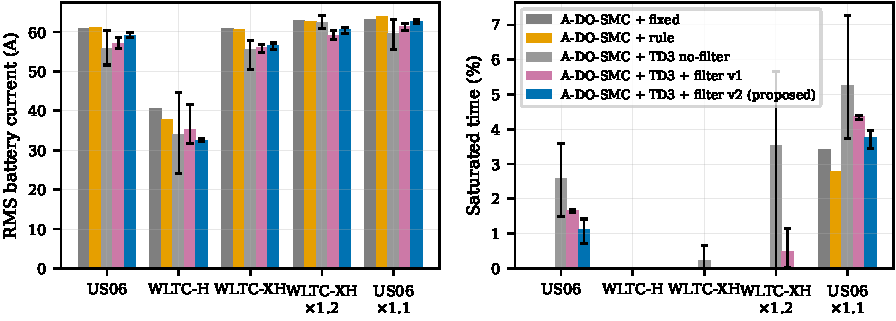
\includegraphics[width=0.9\textwidth]{../results/figures/F5_test_battery_rms_saturation.pdf}
\caption{Held-out test cycles: RMS battery current (left) and fraction of time with the total-current command saturated, i.e., a power deficit (right). Learned supervisors: bar = mean over three training seeds, whisker = min--max.}
\label{fig:testbars}
\end{figure*}

\paragraph{Cycles inside the training power envelope}
On WLTC high and WLTC extra-high, the proposed supervisor (TD3 + filter v2) lowers the RMS battery current in all nine seed pairs, with no saturation:
\begin{itemize}
\item WLTC high: from \R{wh:afix:ibrms}\,A (fixed) and \R{wh:arule:ibrms}\,A (SOC rule) to \R{wh:v2:ibrms:mean}\,A, i.e., \R{wh:v2vsafix:dibrmsabs}\,\% lower than fixed and \R{wh:v2vsarule:dibrmsabs}\,\% lower than the rule;
\item WLTC extra-high: \R{wxa:v2vsafix:dibrmsabs}\,\% lower than fixed.
\end{itemize}
The bus voltage is unaffected: \R{wh:v2:maxdev:mean}\,V versus \R{wh:afix:maxdev}\,V on WLTC high. The price is a higher RMS rate of change of the battery current: \R{wxa:v2vsafix:dslew}\,\% versus fixed on WLTC extra-high.

\paragraph{How the agent achieves this}
The raw logs show that the agents do not use $v_{sc,ref}$ as a slowly varying reserve setpoint, which is how it was intended to be used. Instead, they move it quickly: its standard deviation within a run is \VrefStdMin--\VrefStdMax\,V. As a result, the recovery term \eqref{eq:prec} is at its $\pm\PrecMax$\,kW limit in \CapFracMin--\CapFracMax\,\% of the samples. With the fixed supervisor, the mean $|P_{rec}|$ is only \PrecWHfixedAbs\,kW on WLTC high. In effect, the agent turns the bounded recovery term into a bang-bang actuator for battery power. On transient cycles it switches this power against the load and so lowers the RMS battery current. The agent also keeps $\tau_b$ near its lower bound for most of the run (Fig.~\ref{fig:us06}), which explains the faster battery-current changes.

\paragraph{US06: out of the training envelope}
On US06, the same behavior is harmful. The SC is depleted by long acceleration phases and needs sustained recharging. Here, the switching policy delivers a mean recovery power of only \PrecUSvtwoMin--\PrecUSvtwoMax\,kW (seeds 11, 22, 33), compared with \PrecUSfixed\,kW for the fixed supervisor, which simply recharges at its limit. The SC voltage therefore falls to \R{us06a:v2:vmin:mean}\,V (fixed: \R{us06a:afix:vmin}\,V), below the power-capability level \eqref{eq:vpow}. The command is saturated \R{us06a:v2:sat:mean}\,\% of the time, whereas the fixed supervisor never saturates, and the bus-voltage excursion reaches \R{us06a:v2:maxdev:mean}\,V. This is not a loss of tier-1 stability, since the loop recovers once the demand falls, but it is an operating failure. The \R{us06a:v2vsafix:dibrmsabs}\,\% lower RMS battery current does not compensate for it.

The reserve bound \eqref{eq:vlo} constrains the \emph{reference} $v_{sc,ref}$, not the SC voltage itself, and it is sized using the largest deficit of the training cycles ($E_{res}=\EresKJ$\,kJ). Neither property protects against a policy that keeps the reference high on average while withholding recharge power.

\paragraph{Loads beyond the rating}
With the load scaled by 1.1 (US06) or 1.2 (WLTC extra-high), the peak demand exceeds the vehicle rating used in \eqref{eq:vpow}. On US06$\times1.1$, every configuration saturates: fixed \R{us06b:afix:sat}\,\%, SOC rule \R{us06b:arule:sat}\,\%, v2 \R{us06b:v2:sat:mean}\,\%. On WLTC extra-high$\times1.2$, v2 avoids saturation, as do the fixed and rule supervisors. It still lowers the RMS battery current by \R{wxb:v2vsafix:dibrmsabs}\,\%, but the SC voltage drops to \R{wxb:v2:vmin:mean}\,V, inside the penalized band of \eqref{eq:reward}.

\paragraph{Comparison with the MPC-EMS baseline}
The optimization-based supervisor solves the same problem as the agent, with the same objective, actions and safety filter, but uses a model instead of learning. It changes the picture in three ways.
\begin{itemize}
\item \emph{Battery stress on transient cycles.} Even with the causal persistence forecast, MPC-EMS lowers the RMS battery current more than the agent on every test cycle. On WLTC high, the agent's RMS current is \R{wh:v2vsmpcp:dibrms}\,\% higher (range \R{wh:v2vsmpcp:dibrmsmin}--\R{wh:v2vsmpcp:dibrmsmax}\,\% over the nine seed pairs). On WLTC extra-high the difference is \R{wxa:v2vsmpcp:dibrms}\,\%, and on US06 \R{us06a:v2vsmpcp:dibrms}\,\%. MPC-EMS also has the lower RMS rate of change of the battery current on WLTC high (\R{wh:mpcp:slew}\,A/s against \R{wh:v2:slew:mean}\,A/s). The reduction in battery stress achieved by the agent is therefore not a benefit of learning: a simple model-based search over the same actions does better.
\item \emph{Power deficits.} MPC-EMS keeps the SC at the lowest reference that the filter allows. Its mean $v_{sc,ref}$ is \MPCVrefMeanMin--\MPCVrefMeanMax\,V with a standard deviation of only \MPCVrefStdMin--\MPCVrefStdMax\,V within a run, against a mean of \VtwoVrefMeanMin--\VtwoVrefMeanMax\,V for the agents. With a \HorMPCP\,s horizon and no terminal value on the SC energy, a low reserve costs nothing in the prediction until a deficit is already inside the horizon. On US06 the SC voltage therefore falls to \R{us06a:mpcp:vmin}\,V, and the command is saturated \R{us06a:mpcp:sat}\,\% of the time (agent: \R{us06a:v2:sat:mean}\,\%; fixed: \R{us06a:afix:sat}\,\%). Perfect load preview does not help, because the horizon is too short to see a long acceleration phase coming: saturation is \R{us06a:mpcv:sat}\,\%. On WLTC extra-high$\times1.2$, persistence MPC-EMS saturates \R{wxb:mpcp:sat}\,\% of the time, whereas the agent and both simple supervisors do not saturate. Preview MPC-EMS drove the bus out of its admissible range in \R{wxb:mpcv:fails} of \R{wxb:mpcv:runs} runs on this cycle.
\item \emph{Overall return.} Measured by the training objective, the agent beats persistence MPC-EMS in \R{us06a:v2vsmpcp:wins} seed pairs on US06 (power deficits) and \R{wxa:v2vsmpcp:wins} on WLTC extra-high (SC voltage down to \R{wxa:mpcp:vmin}\,V, inside the penalized band), but in \R{wh:v2vsmpcp:wins} pairs on WLTC high.
\end{itemize}
The comparison sharpens the diagnosis of Section~\ref{sec:discussion}. Two different optimizers, one learned and one model-based, both converge to depleting the SC when the objective does not value the stored energy beyond a short window. The deficits are therefore a property of the problem formulation (objective, horizon and filter), not only of the learning algorithm.

\begin{figure*}[t]
\centering
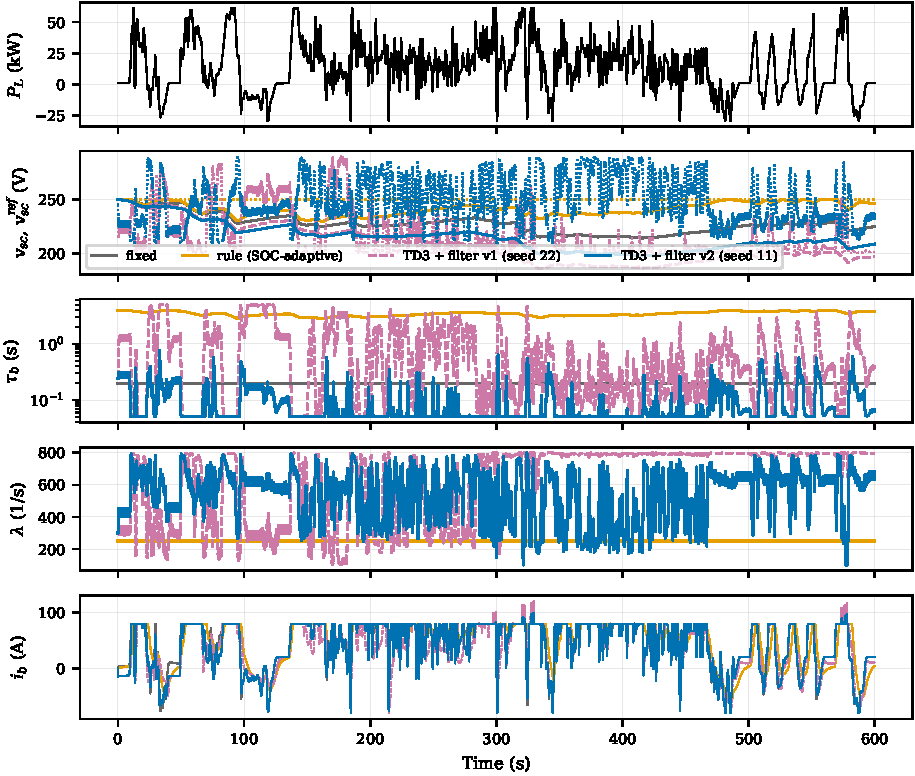
\includegraphics[width=\textwidth]{../results/figures/F4_us06_supervision.pdf}
\caption{US06 (held-out): load power, SC voltage (solid) with its reference (dotted), supervisory parameters $\tau_b$ and $\lambda$, and battery current for the fixed and SOC-rule supervisors and the median-validation agents of filter v1 and v2. The learned agents switch $v_{sc,ref}$ rapidly, so the recovery power is mostly at its $\pm\PrecMax$\,kW limit, and they keep $\tau_b$ near its lower bound. Filter v2 keeps $v_{sc,ref}\ge\VloVtwo$\,V, yet the net recharge is lower than with the fixed supervisor and the SC voltage falls below the level needed to supply the demand.}
\label{fig:us06}
\end{figure*}

\subsection{Effect of the safety filter}\label{sec:res_filter}
The filter changes the failure behavior more than the average performance.
\begin{itemize}
\item \emph{No filter.} One of the three seeds drove the bus out of its admissible range (simulation terminated) on US06, US06$\times1.1$, and WLTC extra-high$\times1.2$. This gives \R{us06a:nof:fails}/9, \R{us06b:nof:fails}/9 and \R{wxb:nof:fails}/9 failed runs. The mean saturation on US06 was \R{us06a:nof:sat:mean}\,\%.
\item \emph{Filter v1.} No run failed; saturation on US06 was \R{us06a:v1:sat:mean}\,\%.
\item \emph{Filter v2.} No agent run failed; saturation on US06 was \R{us06a:v2:sat:mean}\,\%. On WLTC extra-high$\times1.2$, saturation dropped from \R{wxb:v1:sat:mean}\,\% (v1) to \R{wxb:v2:sat:mean}\,\%.
\item \emph{Filter v2 with MPC-EMS.} The same filter did not prevent bus collapse for preview MPC-EMS on WLTC extra-high$\times1.2$ (\R{wxb:mpcv:fails}/\R{wxb:mpcv:runs} runs). The absence of failures in the agent runs is therefore an empirical result for these policies, not a guarantee provided by the filter.
\end{itemize}
The filter also narrows the spread between seeds (Table~\ref{tab:test}). On the main test cycles, the filter modified the $v_{sc,ref}$ component of the action in \FiltVscMin--\FiltVscMax\,\% of the decisions, through the rate limit or the bounds, which reflects the fast switching described above.

\subsection{Additional held-out cycles}\label{sec:res_extra}
\begin{table*}[t]
\centering\footnotesize\setlength{\tabcolsep}{4pt}
\caption{Additional held-out cycles, evaluated only after filter v2 was fixed (one noise seed; learned supervisors: mean $\pm$ standard deviation over three training seeds).}
\label{tab:extra}
\resizebox{\textwidth}{!}{%
\begin{tabular}{@{}llrrrrrc@{}}
\toprule
Cycle & Supervisor (tier 1 = A-DO-SMC) & max$|e|$ (V) & RMS $i_b$ (A) & RMS $\dot\imath_b$ (A/s) & Sat. (\%) & min $v_{sc}$ (V) & Failed runs\\
\midrule
WMTC & Fixed $\theta$ & \R{wmtc:afix:maxdev} & \R{wmtc:afix:ibrms} & \R{wmtc:afix:slew} & \R{wmtc:afix:sat} & \R{wmtc:afix:vmin} & 0\\
 & SOC rule~\cite{nguyen2021adaptive} & \R{wmtc:arule:maxdev} & \R{wmtc:arule:ibrms} & \R{wmtc:arule:slew} & \R{wmtc:arule:sat} & \R{wmtc:arule:vmin} & 0\\
 & TD3 + filter v1 & \R{wmtc:v1:maxdev:mean}\,{\scriptsize$\pm$\R{wmtc:v1:maxdev:std}} & \R{wmtc:v1:ibrms:mean}\,{\scriptsize$\pm$\R{wmtc:v1:ibrms:std}} & \R{wmtc:v1:slew:mean}\,{\scriptsize$\pm$\R{wmtc:v1:slew:std}} & \R{wmtc:v1:sat:mean}\,{\scriptsize$\pm$\R{wmtc:v1:sat:std}} & \R{wmtc:v1:vmin:mean}\,{\scriptsize$\pm$\R{wmtc:v1:vmin:std}} & \R{wmtc:v1:fails}/\R{wmtc:v1:runs}\\
 & TD3 + filter v2 (prop.) & \R{wmtc:v2:maxdev:mean}\,{\scriptsize$\pm$\R{wmtc:v2:maxdev:std}} & \R{wmtc:v2:ibrms:mean}\,{\scriptsize$\pm$\R{wmtc:v2:ibrms:std}} & \R{wmtc:v2:slew:mean}\,{\scriptsize$\pm$\R{wmtc:v2:slew:std}} & \R{wmtc:v2:sat:mean}\,{\scriptsize$\pm$\R{wmtc:v2:sat:std}} & \R{wmtc:v2:vmin:mean}\,{\scriptsize$\pm$\R{wmtc:v2:vmin:std}} & \R{wmtc:v2:fails}/\R{wmtc:v2:runs}\\
\midrule
FTP-MC1b & Fixed $\theta$ & \R{ftp:afix:maxdev} & \R{ftp:afix:ibrms} & \R{ftp:afix:slew} & \R{ftp:afix:sat} & \R{ftp:afix:vmin} & 0\\
 & SOC rule~\cite{nguyen2021adaptive} & \R{ftp:arule:maxdev} & \R{ftp:arule:ibrms} & \R{ftp:arule:slew} & \R{ftp:arule:sat} & \R{ftp:arule:vmin} & 0\\
 & TD3 + filter v1 & \R{ftp:v1:maxdev:mean}\,{\scriptsize$\pm$\R{ftp:v1:maxdev:std}} & \R{ftp:v1:ibrms:mean}\,{\scriptsize$\pm$\R{ftp:v1:ibrms:std}} & \R{ftp:v1:slew:mean}\,{\scriptsize$\pm$\R{ftp:v1:slew:std}} & \R{ftp:v1:sat:mean}\,{\scriptsize$\pm$\R{ftp:v1:sat:std}} & \R{ftp:v1:vmin:mean}\,{\scriptsize$\pm$\R{ftp:v1:vmin:std}} & \R{ftp:v1:fails}/\R{ftp:v1:runs}\\
 & TD3 + filter v2 (prop.) & \R{ftp:v2:maxdev:mean}\,{\scriptsize$\pm$\R{ftp:v2:maxdev:std}} & \R{ftp:v2:ibrms:mean}\,{\scriptsize$\pm$\R{ftp:v2:ibrms:std}} & \R{ftp:v2:slew:mean}\,{\scriptsize$\pm$\R{ftp:v2:slew:std}} & \R{ftp:v2:sat:mean}\,{\scriptsize$\pm$\R{ftp:v2:sat:std}} & \R{ftp:v2:vmin:mean}\,{\scriptsize$\pm$\R{ftp:v2:vmin:std}} & \R{ftp:v2:fails}/\R{ftp:v2:runs}\\
\midrule
Long-haul (first 1200\,s) & Fixed $\theta$ & \R{lh:afix:maxdev} & \R{lh:afix:ibrms} & \R{lh:afix:slew} & \R{lh:afix:sat} & \R{lh:afix:vmin} & 0\\
 & SOC rule~\cite{nguyen2021adaptive} & \R{lh:arule:maxdev} & \R{lh:arule:ibrms} & \R{lh:arule:slew} & \R{lh:arule:sat} & \R{lh:arule:vmin} & 0\\
 & TD3 + filter v1 & \R{lh:v1:maxdev:mean}\,{\scriptsize$\pm$\R{lh:v1:maxdev:std}} & \R{lh:v1:ibrms:mean}\,{\scriptsize$\pm$\R{lh:v1:ibrms:std}} & \R{lh:v1:slew:mean}\,{\scriptsize$\pm$\R{lh:v1:slew:std}} & \R{lh:v1:sat:mean}\,{\scriptsize$\pm$\R{lh:v1:sat:std}} & \R{lh:v1:vmin:mean}\,{\scriptsize$\pm$\R{lh:v1:vmin:std}} & \R{lh:v1:fails}/\R{lh:v1:runs}\\
 & TD3 + filter v2 (prop.) & \R{lh:v2:maxdev:mean}\,{\scriptsize$\pm$\R{lh:v2:maxdev:std}} & \R{lh:v2:ibrms:mean}\,{\scriptsize$\pm$\R{lh:v2:ibrms:std}} & \R{lh:v2:slew:mean}\,{\scriptsize$\pm$\R{lh:v2:slew:std}} & \R{lh:v2:sat:mean}\,{\scriptsize$\pm$\R{lh:v2:sat:std}} & \R{lh:v2:vmin:mean}\,{\scriptsize$\pm$\R{lh:v2:vmin:std}} & \R{lh:v2:fails}/\R{lh:v2:runs}\\
\bottomrule
\end{tabular}}
\end{table*}


Table~\ref{tab:extra} reports three cycles that were introduced after filter v2 was fixed and influenced no design choice.
\begin{itemize}
\item \emph{WMTC.} v2 lowers the RMS battery current by \R{wmtc:v2vsafix:dibrmsabs}\,\% (fixed) and \R{wmtc:v2vsarule:dibrmsabs}\,\% (rule) without saturation, whereas v1 saturated \R{wmtc:v1:sat:mean}\,\% of the time.
\item \emph{FTP-MC1b} (mild). The reduction is \R{ftp:v2vsafix:dibrmsabs}\,\% (fixed) and \R{ftp:v2vsarule:dibrmsabs}\,\% (rule).
\item \emph{Long-haul segment} (mostly steady cruising). The agent \emph{increases} the RMS battery current from \R{lh:afix:ibrms}\,A to \R{lh:v2:ibrms:mean}\,A (+\R{lh:v2vsafix:dibrms}\,\%). The same switching of $P_{rec}$ between $\pm\PrecMax$\,kW now has no transient to cancel. It therefore adds a square-wave component of about $\PrecMax\,\mathrm{kW}/\SI{300}{V}\approx\SI{17}{A}$ to an otherwise nearly constant battery current; with the fixed supervisor, the mean $|P_{rec}|$ is \PrecLHfixedAbs\,kW.
\end{itemize}
This is a second, different failure mode outside the training distribution. MPC-EMS does not show it: on the long-haul segment its RMS battery current is \R{lh:mpcp:ibrms}\,A (persistence), below the \R{lh:afix:ibrms}\,A of the fixed supervisor, because switching $P_{rec}$ brings no predicted benefit when the load is nearly constant. Among the causal supervisors, persistence MPC-EMS also gives the lowest RMS battery current on FTP-MC1b (\R{ftp:mpcp:ibrms}\,A) and WMTC (\R{wmtc:mpcp:ibrms}\,A). On WMTC, however, it saturates \R{wmtc:mpcp:sat}\,\% of the time with a bus excursion of \R{wmtc:mpcp:maxdev}\,V, whereas the agent does not saturate.

\subsection{Computational cost}\label{sec:res_cost}
On the simulation host, one tier-1 update (compiled) costs \TimeADOSMC\,\si{\micro s}. One tier-2 decision (actor with \NActorParams\ parameters plus safety filter, interpreted Python) costs \TimeAgent\,\si{\micro s} every \SI{100}{ms}. One MPC-EMS decision (\NCandMPC\ candidates, \HorMPCP\,s horizon, vectorized NumPy) has a median cost of \TimeMPCEMS\,ms, more than an order of magnitude above the actor but still only about 1\,\% of the decision period. Both figures are relative indicators only; execution on an automotive microcontroller was not measured.

